% TEMPLATE for Usenix papers, specifically to meet requirements of
%  USENIX '05
% originally a template for producing IEEE-format articles using LaTeX.
%   written by Matthew Ward, CS Department, Worcester Polytechnic Institute.
% adapted by David Beazley for his excellent SWIG paper in Proceedings,
%   Tcl 96
% turned into a smartass generic template by De Clarke, with thanks to
%   both the above pioneers
% use at your own risk.  Complaints to /dev/null.
% make it two column with no page numbering, default is 10 point

% Munged by Fred Douglis <douglis@research.att.com> 10/97 to separate
% the .sty file from the LaTeX source template, so that people can
% more easily include the .sty file into an existing document.  Also
% changed to more closely follow the style guidelines as represented
% by the Word sample file. 

% Note that since 2010, USENIX does not require endnotes. If you want
% foot of page notes, don't include the endnotes package in the 
% usepackage command, below.

% This version uses the latex2e styles, not the very ancient 2.09 stuff.
\documentclass[letterpaper,twocolumn,10pt]{article}
\usepackage{usenix,epsfig,endnotes}

%%%%%%%%%%%%%%%%%%%%%%%%%%%%%%%%%%%%
% Accents français
%%%%%%%%%%%%%%%%%%%%%%%%%%%%%%%%%%%%
\usepackage[utf8]{inputenc}
\usepackage[american]{babel}
\usepackage[T1]{fontenc}

\usepackage{xspace}
\usepackage[hyphens]{url}
\usepackage{hyperref}
\hypersetup{breaklinks=true}
\usepackage[capitalise, noabbrev]{cleveref}

%%%%%%%%%%%%%%%%%%%%%%%%%%%%%%%%%%%%
% Todo notes
%%%%%%%%%%%%%%%%%%%%%%%%%%%%%%%%%%%%
\usepackage[textwidth=17mm]{todonotes}
\newcommand{\customtodo}[4]{
        \todo[color=#2,inline,size=\small]{
                \ifx&#3&
                        \textbf{#1} #4
                \else
                        \textbf{#1$\Rightarrow$#3} #4
                \fi
        }
}
\newcommand{\AL}[2][]{\customtodo{AL}{green!50}{#1}{#2}}
\newcommand{\ALm}[1]{\todo[color=green!50,size=\small]{#1}}
\newcommand{\JM}[2][]{\customtodo{JM}{red!20}{#1}{#2}}
\newcommand{\JMm}[1]{\todo[color=red!15,size=\small]{#1}}
\newcommand{\FW}[2][]{\customtodo{FW}{brown!20}{#1}{#2}}
\newcommand{\RAC}[2][]{\customtodo{RAC}{yellow!15}{#1}{#2}}
\newcommand{\RACm}[1]{\todo[color=yellow!15,size=\small]{#1}}
\newcommand{\DPm}[1]{\todo[color=yellow!15,size=\small]{#1}}
\newcommand{\DP}[2][]{\customtodo{DP}{yellow!15}{#1}{#2}}


\newcommand{\ie}[0]{{\em i.e.},\xspace}
\newcommand{\vs}[0]{{\em vs.}\xspace}
\newcommand{\eg}[0]{{\em e.g.},\xspace}
\newcommand{\etal}[0]{{\em et al.}\xspace}
\newcommand{\wrt}[0]{{\em w.r.t.}\xspace}
\newcommand{\aka}[0]{{\em a.k.a.}\xspace}
\newcommand{\via}[0]{{\em via}\xspace}

\newcommand{\cloud}{cloud\xspace}
\newcommand{\clouds}{clouds\xspace}
\newcommand{\fog}{fog\xspace}
\newcommand{\edge}{edge\xspace}
\newcommand{\computing}{computing\xspace}
\newcommand{\extreme}{extreme\xspace}
\newcommand{\edgecomputing}{\edge\computing}
\newcommand{\extremeedge}{\extreme\edge}
\newcommand{\cloudcomputing}{\cloud\computing}

%%%%%%%%%%%%%%%%%%%%%%%%%
% Table add-ons
%\usepackage{array,multirow}
\usepackage{longtable, booktabs, multirow}
\usepackage{array,booktabs}
\newcolumntype{L}{@{}>{\kern\tabcolsep}l<{\kern\tabcolsep}}
\usepackage{colortbl}

\newcolumntype{P}[1]{>{\centering\arraybackslash}p{#1}}
\newcolumntype{M}[1]{>{\centering\arraybackslash}m{#1}}

\newcommand{\Tstrut}{\rule{0pt}{2.75ex}\rule[-1.5ex]{0pt}{0pt}}
\newcommand{\Bstrut}{\rule{0pt}{1.5ex}\rule[-1.5ex]{0pt}{0pt}}
\newcommand{\Rstrut}{\rule{0pt}{1.75ex}\rule[-1.25ex]{0pt}{0pt}}

\newcommand{\thickhline}{\noalign{\hrule height 1.5pt}}

\sloppy

\usepackage{url}
\usepackage{paralist}
\usepackage[loose]{subfigure}

% listing preference
\usepackage[scaled=0.85]{beramono}
\usepackage{listings}
\lstset{numbers=none,basicstyle=\ttfamily}
\usepackage{import}


\usepackage{enumitem}


\begin{document}

%don't want date printed
\date{}

%make title bold and 14 pt font (Latex default is non-bold, 16 pt)
\title{\Large \bf Top-Down/Bottom-Up: How Designing a Resource Management System in Charge Of Operating Edge Computing Infrastructures}

%for single author (just remove % characters)
\author{
{\rm Your N.\ Here}\\
Your Institution
\and
{\rm Second Name}\\
Second Institution
% copy the following lines to add more authors
% \and
% {\rm Name}\\
%Name Institution
} % end author

\maketitle

% Use the following at camera-ready time to suppress page numbers.
% Comment it out when you first submit the paper for review.
\thispagestyle{empty}


\subsection*{Abstract}
Your Abstract Text Goes Here.  Just a few facts.
Whet our appetites\endnote{Remember to use endnotes, not footnotes!}.
        
\vspace*{-.2cm}
\section{Introduction}
\label{sec:intro}

\vspace*{-.1cm}

% % Edge Infrastructures are the next platform
% With the emergence of Network Function Virtualization (NFV)
% technologies as well as Internet of Things (IoT) and augmented/virtual
% reality (AR/VR) applications, Cloud and Network communities are
% advocating for going towards massively distributed small sized
% infrastructures that are deployed at the edge of the network.
% %
% Referred to as the Edge Computing paradigm, this model aims at
% delivering Cloud Computing capabilities closer to end-users, their
% related devices, and applications.
% %

While several academic studies have been highlighting the advantages
of the \edgecomputing paradigm in various
domains~\cite{bonomi2012fog,satyanarayanan2017emergence,shi2016edge,yi2015fog,zhang2015cloud},
%%
progress on how to operate and use infrastructures that serve it are marginal.
Current solutions like Akamai Cloudlets~\cite{akamai:cloudlets} or
AWS Lambda~\cite{amazon:lambda-edge} are close to the initial \fog proposal that
allows to run domain-specific applications on NFV-enabled infrastructures (at
the \edge) and centralized \clouds~\cite{bonomi2012fog}.
%In other words,
%current Edge Infrastructure-as-a-Service (IaaS)
%
Since these solutions do not allow to run stateful workloads in isolated
environments (e.g. containers, virtual machines (VM)) they do not fit the
requirements expected by software developers and operators (DevOps) who expect
to find most features that made current \cloudcomputing solutions successful
also at the \edge (such approaches are not considered in this paper).
%These solution do not allow to run stateful workloads in isolated environments
%such as containers or virtual machines (and are thus out of the scope of this
%paper).
%%
%This would come as a surprise for software developers and operators (DevOps)
%that will expect to find most features that made current \cloudcomputing
%solutions successful also at the \edge.

% Our community should tackle the challenge of delivering a general
% resource management system to operate and use Edge Computing
% infrastructure. Something that will first, let an operator aggregates,
% supervises and exposes the massively distributed resources of the
% infrastructure and second, let a developer implements new kinds of
% services on top of that infrastructure that may be deployed and
% managed on demand.

%% Thus, the development of a general resource management system to
%% operate and use Edge Computing infrastructures is still an open
%% question.

%% %%  We need a resource management system that enables administrators to
%% %% operate and end-users to use edge resources.
%% %% a resource management system that will enable, on the one hand,
%% %% an operator to aggregate, supervise and expose such massively
%% %% distributed resources and, on the other hand, a developer to implement
%% %% new kinds of services that may be deployed and managed on demand is
%% %% still an open question.

%% %%  Delivierng en Edge IaaS system is complex
%% Domain specific solutions~\cite{bonomi2012fog} allow IoT applications
%% to run on infrastructures composed of NFV-enabled hardware (at the
%% edge) and existing centralized clouds. However, these solutions do not
%% allow to run workloads in isolated environments such as containers or
%% virtual machines (VMs).
%% %
%% This is rather critical as developers/end-users expect to find
%% most features that makes the success of current Cloud Computing solutions.

%% Requirements:
%%
%% 1. il y a des fonctionnalités spécifiques au edge
%%
%% 2. on a étudié différentes stratégies de design d'une IaaS manager
%%    qui implementerait nos requieremtn avec comme *contraintes de
%%    réutilier au plus les VIM*.

%% Les implem essaye de réutiliser les VIM pour minimiser l'effort de
%% dvlp. Elle font ceci par aggrega des API, mais le problème est
%% qu'elles se limite à être des gestionnaires de resources (cf k8s
%% discussion avec Adrien) alors que un VRAIE IaaS manager doit
%% considérer plus de chose (donner un exemple de req).

%On this basis,
%
The ETSI Mobile Edge Computing Industry Specification Group
defined in 2016 an architecture to orchestrate distinct
independent \cloud systems, \aka Virtual
Infrastructure Managers (VIM) ~\cite{7574435}.
%
The idea consists in federating VIMs of the different Data Centers (DCs) that
compose the \edge infrastructure.  By reusing VIMs, ETSI targets an
\edgecomputing
resource management that behaves in a same fashion as traditional ones, 
while mitigating development requirements.
%
Although there is no implementation available, the idea of federating
VIMs seems promising as several projects have been built on similar
concepts. ONAP~\cite{onap}, an industry-driven solution,
enables the orchestration and automation of virtual network functions
across distinct VIMs. From the academic side, FogBow~\cite{brasileiro2016fogbow} aims to support federations
of Infrastructure-as-a-Service (IaaS) providers. More recently, NIST
initiated a collaborative effort with IEEE to advance Federated
\cloud through the development of a conceptual architecture and a
vocabulary\endnote{\url{https://collaborate.nist.gov/twiki-cloud-computing/bin/view/CloudComputing/FederatedCloudPWGFC}
  (March 2018).}.

Although all these projects provide valuable contributions, they all have
been designed by only considering the DevOps' perspective. They provide
abstractions to manage the life cycle of geo-distributed applications,
but do not address administrative requirements.
%
However, \edgecomputing infrastructures differ from federated \cloud systems
in various aspects~\cite{openstack:whitepaper}, for instance:
\edge sites are potentially unmanned and therefore must be administered remotely;
management systems should be designed to cope with intermittent network access to sites; distinct operators might be interested in interconnecting their infrastructures (like network peering).
%

To capitalize on the advent of \edgecomputing, our community should take part
of current discussions and actions in order to deliver a well-suited
resource management system. A system that will first, let an operator aggregate, supervise and expose the massively distributed resources of the infrastructure,
and second, let DevOps implement new kinds of services on top of an infrastructure that may be deployed and managed on-demand.

% Designing and implementing a complete software stack to enable
% administrators to operate, and developers to use, distinct edge sites
% like a global Cloud Computing infrastructure is a difficult challenge
% for our community. However it is a challenge we should tackle soon to
% favor the advent of the Edge Computing paradigm.

In this paper, we present reflections to initiate discussions through our community.

\begin{itemize}[noitemsep, topsep=0pt]
\item First, we introduce a classification of the features expected by
  both administrators and DevOps. This classification is valuable to
  identify missing mechanisms in resource management systems.
 % Moreover, it should deliver significant insights on the
 % design and implementation of a resource management system for the
 % edge computing.
\item Second, based on the identified requirements, we discuss
  how an \edge resource management system
  should be designed. In particular, we study \emph{pros} and
  \emph{cons} of \emph{top-down} and \emph{bottom-up} approaches. The
  former consists in interacting with each site only through
  exposed VIM APIs, such as in federated approaches. The
  latter aims at revising internal mechanisms of VIMs to enable native
  collaborations.
  \end{itemize}

\begin{figure}[t]
  \centering
  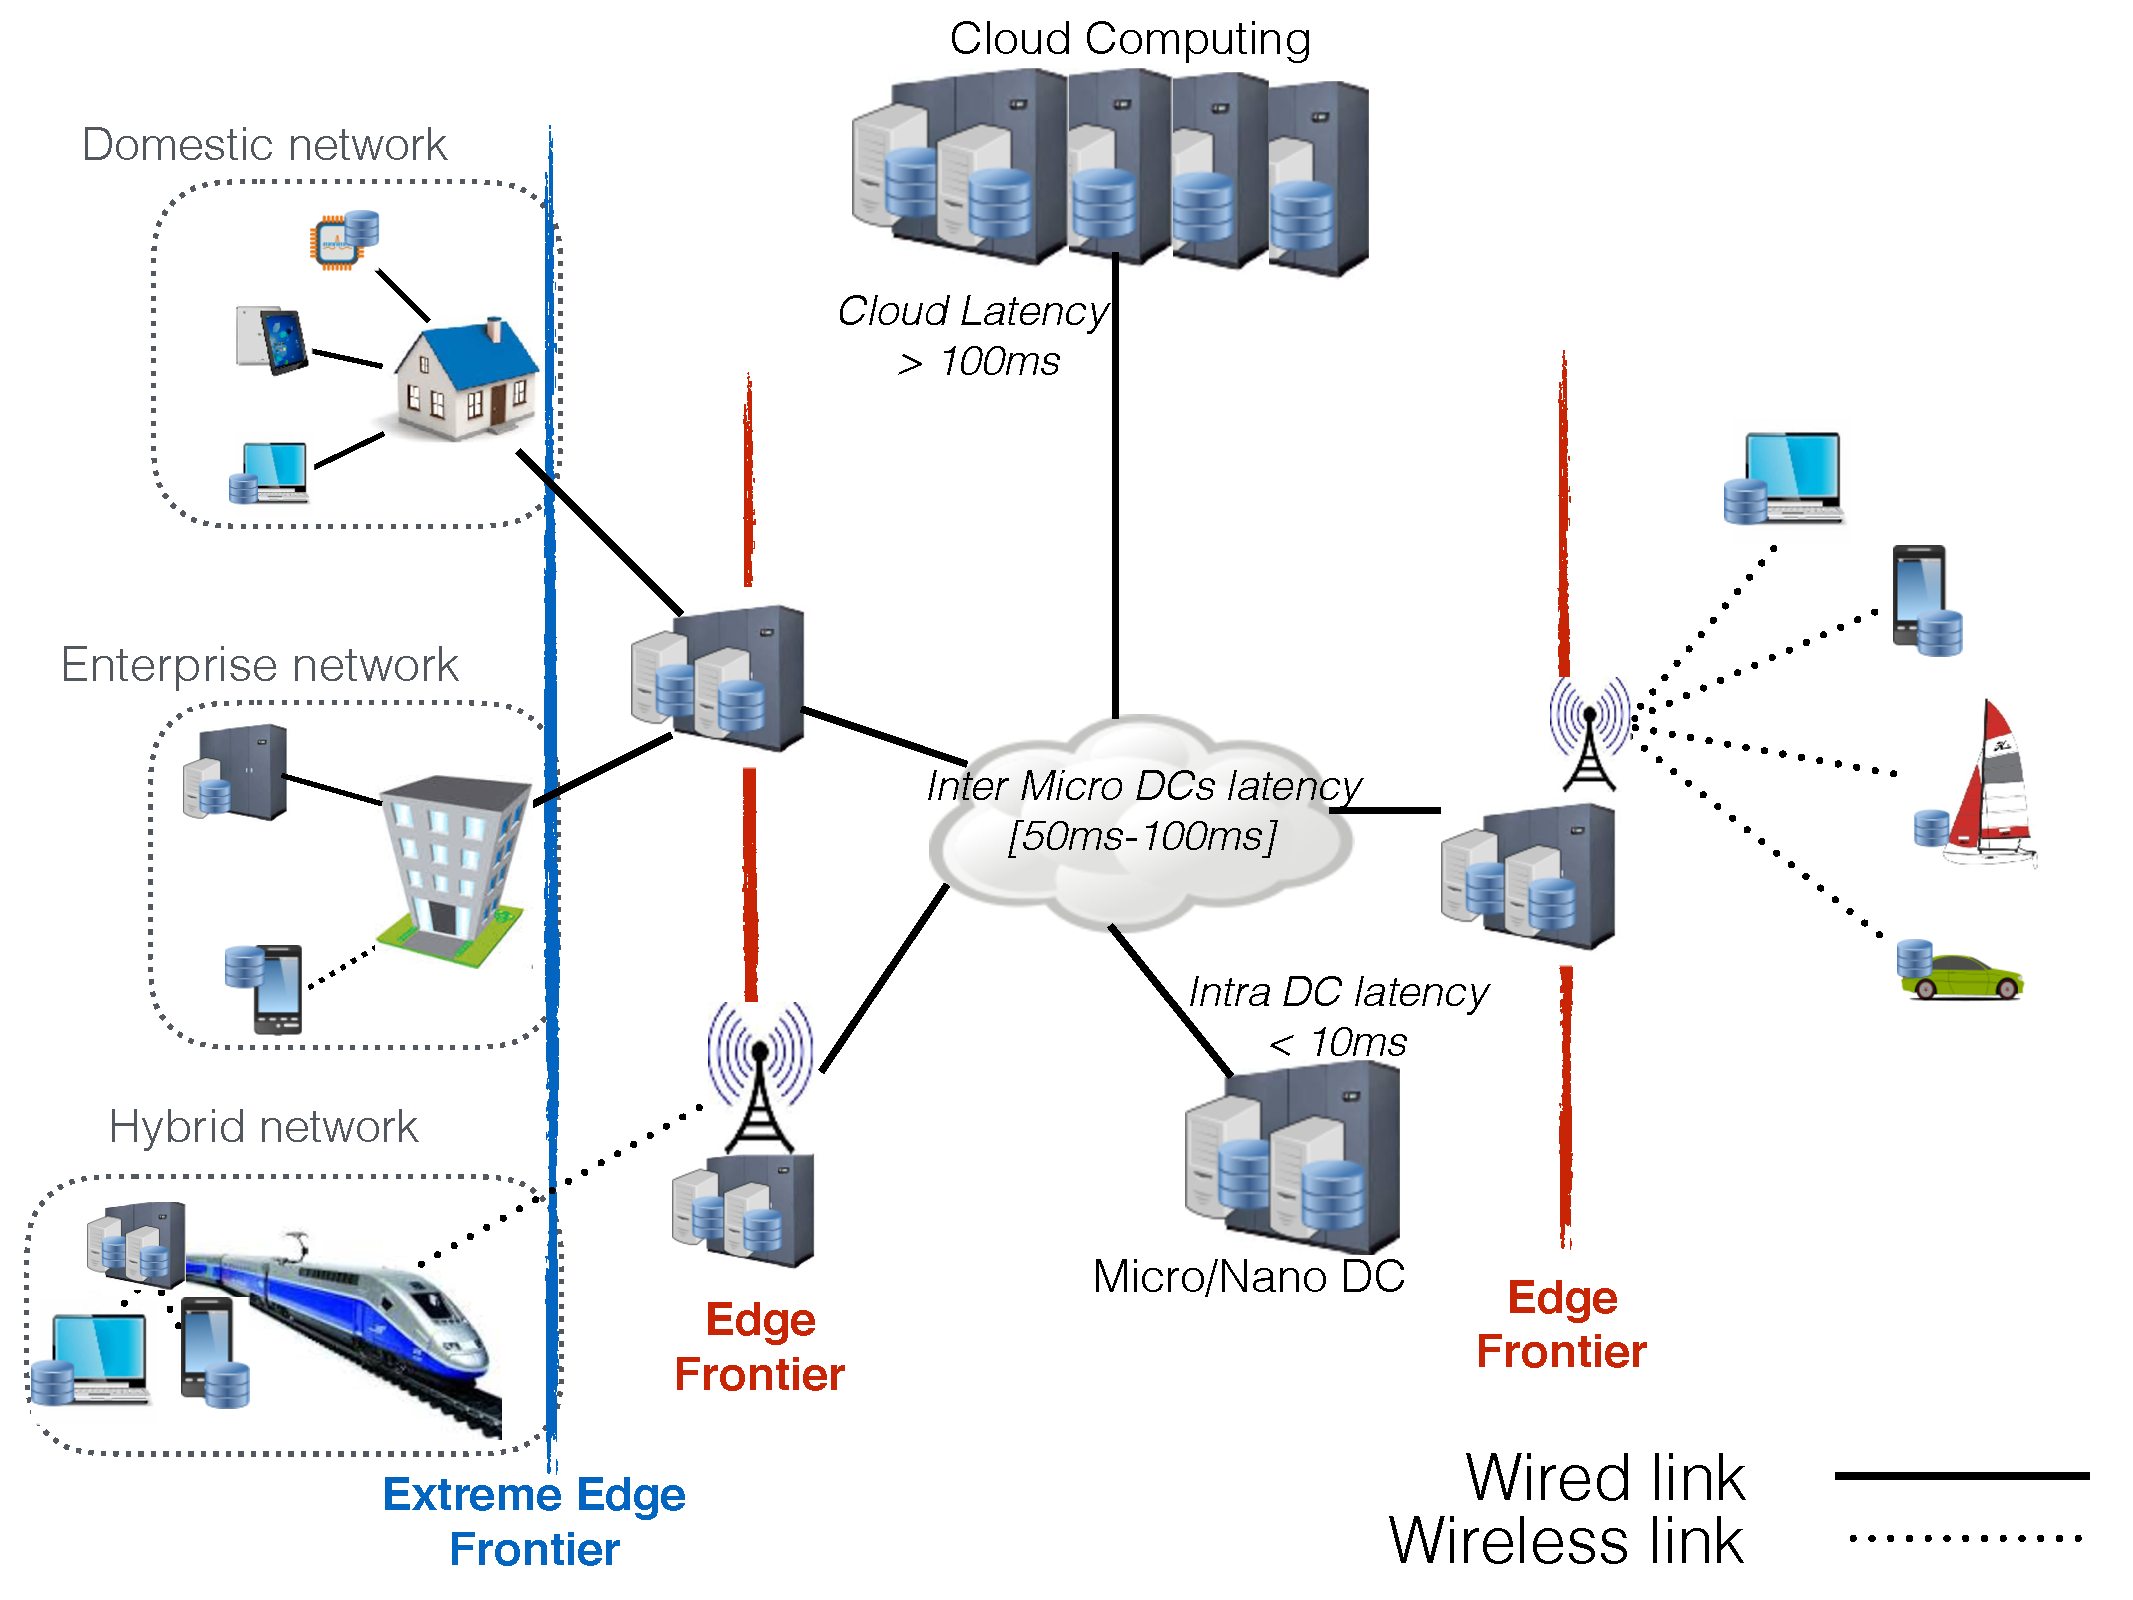
\includegraphics[width=.95\columnwidth]{./figures/figure_fog.pdf}
    \vspace*{-.2cm}
  \caption{Edge Computing Infrastructure~\cite{7923796}.}
    {\small The red dashed lines depict a split-brain situation that isolates
    \emph{Site 1} from other sites.}
  \label{fig:fogedge-archi}
  \vspace*{-.3cm}
\end{figure}

%From the hardware viewpoint,
Since there are as many \edge infrastructures as
use-cases, we highlight that the infrastructure considered in this study is
composed of several individually-managed and geo-distributed micro DCs (up to
thousands) composed of up to one hundred servers (nearly two racks).
Figure~\ref{fig:fogedge-archi} depicts such an infrastructure. The expected
latency and bandwidth between elements may fluctuate, in particular because
networks can be wired or wireless. Moreover, disconnections between sites may
occur, leading to network split-brain situations~\cite{4456903}.
Finally, it is possible to consider additional DCs at the \extremeedge, within private institutions or public transports.
%
From the software viewpoint, since we investigate how existing \cloud managers
can be extended to the \edge, we consider as our default VIM
OpenStack~\cite{openstack:www}: the de-facto open-source solution for
\cloudcomputing infrastructures.%
\endnote{One can note however that our study applies on any other resource
manager built on the similar building blocks as OpenStack (\eg Kubernetes).
Such building blocks are conceptually identified
in~\cite{moreno2012csp}.}

%From the software viewpoint, to simplify the model and without loss of
%generality, we mainly assume OpenStack ~\cite{openstack:www} as the default
%VIM.

%After years of development, OpenStack is today the de facto open-source solution to operate, supervise and use
%IaaS infrastructures.
%More recently it has increased its effort to address edge computing cases.
%The OpenStack community gathers more than 500
%organizations, including large groups, in particular key actors of
%edge infrastructures such as ATT, Verizon~\ldots.

The remainder of the paper is organized as follows.
Section~\ref{sec:requirements} provides a list of features expected by administrators
and DevOps.
%highlighting in particular differences \wrt federated infrastructures.
Section~\ref{sec:system_design_considerations} studies how OpenStack satisfies
these features, highlighting the need for collaboration across the
entire \edge infrastructure. Section~\ref{sec:design_discussion} discusses two
approaches to design a resource management system for the \edge.
Section~\ref{sec:conclusion} concludes the paper.

% In this paper, we provide a list of expected features for both administrators and admins.
% We investigate whether a stack such as OpenStack, the defacto open-source standard can fullfil these requirements
% We finally discusss two possibles ways for moving forward: top/down vs bottom/up.

\vspace*{-.2cm}



\section{Admin/Devops' Requirements}
\label{sec:requirements}

% \begin{figure}[t]
%   \centering
%   \def\svgwidth{\columnwidth}
%   \input{figures/sites.pdf_tex}
%   \caption{Partial representation of the targeted Edge infrastructure, composed
%     of multiple sites. Each site is composed of many servers (represented by
%     black bullets) and have a set of users (depicted by black squares). The red
%     dashed line depicts a split-brain situation that separates the
%     infrastructure into $2$ partitions, isolating \emph{Site 1} from \emph{Site
%     2} and \emph{3}.}
%   \label{fig:fogedge-archi}
% \end{figure}

\begin{table*}
    \centering
        
\scriptsize
\begin{tabular}{@{} l L L L @{} >{\kern\tabcolsep}l @{}}
    \toprule
  %\begin{tabular}{@{} p{.25\textwidth} p{.25\textwidth}p{.25\textwidth}p{.25\textwidth} @{} >{\kern\tabcolsep}l @{}}    \toprule

    \emph{Levels} & \emph{Admin}& \emph{User} & \emph{Both} \\
    \midrule

    L1: Operate/use any site &
    Manage any site: &
    Provision on-demand on any site: &
    Collect metrics regarding a single site: \\ 

    (all operations are based in single site) &
    - install services &
    - compute resources&
    Security (secured communications, \\

    &
    - use services (users, flavors, quotas)&
    - network resources&
    auditing, integrity)\\

    &
    - upgrade services&
    - storage resources&
    Resiliency\\
    %\\% add space between levels

    \rowcolor{black!20}[0pt][0pt]
    L2: Operate/use several sites &
    &
    &
    L1 but over a set of sites\\

    \rowcolor{black!20}[0pt][0pt]
    (all operations cover at least two sites) &
    &
    &
    Collect metrics regarding many sites\\

    \rowcolor{black!20}[0pt][0pt]
    - L2.1 Explicit manner&
    Manage a specific set of sites &
    Provision on a specific set of sites &
    \\
    
    \rowcolor{black!20}[0pt][0pt]
    - L2.2 Implicit manner&
    Cross-site Autonomous management&
    Cross-site Autonomous provisioning&
    \\
    %\\% add space between levels

    L3: Robustness \wrt split brains &
    &
    &
    L1 for an isolated site\\ 

    (all operations cover one or many sites) &
    &
    &
    L1 and L2 for an isolated set of sites\\

    - L3.1 Application robustness&
    \hfill ------ \hfill &
    Access user's applications&
    Collect metrics regarding one or many sites\\

    - L3.2 Management service robustness&
    Manage one or many sites &
    Provision on one or many sites&
    \\
    %\\% add space between levels

    \rowcolor{black!20}[0pt][0pt]
    L4: Multiple Cloud environments &
    &
    &
    L3 with different types of IaaS managers\\ 

    \rowcolor{black!20}[0pt][0pt]
    (all operations cover one or many sites) &
    &
    &
    Discover sites' capabilities/compatibilities\\

    \rowcolor{black!20}[0pt][0pt]
    - L4.1 Different IaaS versions&
    Manage different IaaS versions&
    Provision on different IaaS versions&
    \\
    
    \rowcolor{black!20}[0pt][0pt]
    - L4.2 Different IaaS technologies&
    Manage different IaaS technos&
    Provision on different IaaS technos&
    \\
    %\\% add space between levels

    L5: Multiple operators &
    \hfill ------ \hfill &
    Provision on one or many sites&
    L4 with multiple operators\\ 

    (all operations cover one or many sites) &
    &
    &
    Collect metrics from different operators\\
    \bottomrule

\end{tabular}


    \caption{Classification of the requirements to administrate and use Edge
    Computing infrastructures in $5$ levels.}
    \label{tab:requirements}
\end{table*}

In this section, we classify features administrators and devops expect
to find in the context of Edge Computing infrastructures.
Our classification is based on $5$ \emph{levels}, starting from the easiest
aspects, \ie interacting with a single site (considered in level 1 or L1), to
more complex aspects like managing multiple sites (L2), up to considering that
sites can be owned by different operators (L5).
\Cref{tab:requirements} summarizes the classification we detail in the following. 

As previously mentioned, a large part of these features are common to
the ones offered by current IaaS resource management systems. They are
implemented by various services, each of which is in charge of the
management of a particular aspect of the infrastructure
%.In this paper, we consider the Compute, Storage and
%Network managers as well as the monitoring and administrative
%tools
~\cite{moreno2012csp}.
\ALm{Not sure whether we should introduce
  service here. Maybe this is something we should only put at the end
  of this section to make a transition with the other ones. The issue
  is that we need it for the moment in L2.}

\paragraph{L1: Operate/use any site}
As depicted in the second row of \cref{tab:requirements}, this level
considers actions both administrators and users expect to perform
when considering a single site, supposing the site is reachable.
%
Most operations are elementary from the Edge viewpoint because they correspond
to the ones already provided by OpenStack for both administrators and devops.
In other words, each Edge site can be considered as an independent Cloud at
this level. The unmanned aspect only impacts this level by requiring to perform
all operations remotely if needed.
%security
Furthermore, the resource management system should provide means to
ensure the integrity of the hardware resources taking part to the Edge
infrastructure. Strategies such as enabling/disabling physical
interactions with the equipment should be considered.

% %
% Regarding administrators,  Administrators should be able to
% install and upgrade the aforementioned resource management
% services. After what, they can use those services to manage
% users, accesses, flavors (\ie available capacities of compute
% resources) and quotas.

% Regarding devops, they should be able to provision compute, network or
% storage resources like any traditional Cloud platform, supposing they
% are authorized to.

% In addition, admins and users share common expectations.
% % collect metrics
% First they want to monitor various metrics related to resources,
% users, and projects . This is used for instance for
% respectively managing quotas and listing existing resources.

\paragraph{L2: Operate/use several sites:}

%% TODO
% For instance, a user of \emph{Site 1} 
In L2, L1 features are considered but over multiple sites (at least two). This
includes operations such as provisioning a resource on a site using resources
from another one, managing several resources or gathering information from
various sites simultaneously.
%(interconnecting two VMs with a dedicated network).
Operations can be either intra-services (same service from different sites) or
inter-services (different services from different sites).

Concrete operations consist for instance in configuring users'
access on a per-site basis, listing available VM images or pushing new
ones on multiple sites (intra-service operations). From the
devops viewpoint, a user should be able to boot a VM on \emph{Site 1} (depicted
on \cref{fig:fogedge-archi}) using an image defined in \emph{Site 2}
(inter-service operation). Similarly to L1, they both expect metrics collected
from several sites and collaborated mechanisms regarding the security (\eg
secret key sharing, network encryption).

Because collaboration between sites can be either explicit (\ie the
targeted sites are explicitly specified in the operation), or implicit
(\ie the resource management system is in charge of selecting
resources), we have defined two sub-levels as depicted in
\cref{tab:requirements}, respectively called L2.1 and L2.2. The implicit
manner suggests that policies (\eg performance objectives, energy
consumption) and constraints (\eg affinity rules, underlying hardware
requirements) are provided by admins and devops so that the resource management
system takes the right decisions regarding the defined desiderata and the state
of the infrastructure (\eg auto-scaling, relocating workloads between sites,
re-scheduling faulty resources across sites).
% should be elaborated and/or refs should be given here

\paragraph{L3: Robustness \wrt network split brains:}
The next level we define is related to the limited or intermittent
network connections between sites. Similarly to the previous level,
L3 includes all L2 operations but with the possibility to face
\emph{network split brains} (\ie, situations where the infrastructure is
partitioned due to communication failures).
%
\Cref{fig:fogedge-archi} depicts such a case where \emph{Site 1} is isolated
from the other sites. In this scenario, administrators/devops that can reach
the site (\ie located in the same geographical area) should be able to perform
L1 operations regarding \emph{Site 1}, even if it is isolated from other sites.
Such a requirement make sense as L1 operations are only related to one site and
thus do not impact the other ones.
%
Regarding the second partition which contains the other sites, L1 and L2
operations must be guaranteed for any subset of sites inside the partition.

Split brains have a distinct impact on already-provisioned resources and on the
management services that enable to provision new resources or change existing
ones. As a consequence, we decided to refine L3 into two sub-classes. L3.1 is
related to the features that allow already-deployed applications to continue to
serve local requests without being impacted. For instance, an \emph{apache}
server or a storage backend should be able to satisfy requests coming from the
same geographical area, even if management services cannot be reached. L3.2
features are related to the provisioning of new resources and other management
operations as described in the previous paragraph.
%
Note that guaranteeing L2 features will not be always possible at the L3.2
level because information cannot be gathered in case of a disconnection. For
instance, guaranteeing quotas across the infrastructure overall is impossible
without relaxing the consistency of the information. New approaches will have
to be proposed for such operations.

Finally, the possibly intermittent network connectivity between Edge resources
requires to have operations that enable sites to join and leave the
infrastructure.

% what about quotas? how to manage them in case of split-brain?
% suppose a user has a global quotas on several sites, it is impossible to
% determine its global consumption in case of split-brains?

\paragraph{L4: Multiple Cloud environments:}
Delivering a resource management system at large scale in a unified manner is
not conceivable from the software viewpoint. Different versions of each
service, and potentially different infrastructure managers in charge of
different sites, will co-exist at the same time across the whole
infrastructure. It is thus important to consider specific requirements to deal
with such a constraint, which we gather in L4.
%
More precisely, L4.1 considers L3 features when Edge sites can be
operated by different versions of the same software stack.
%
L4.2 increases the complexity by adding into the big picture the
possibility to deal with different resource management systems,
including possibly different concepts (\eg OpenStack for VMs and
Kubernetes for Containers).

As a consequence, it is necessary to discover sites' capabilities to
determine their relationship in order to only allow possible operations.

\paragraph{L5: Multiple operators:}
L5 corresponds to the holy grail in terms of expected features. In
addition to L4 features, it includes the possibility to use sites
owned by different operators. As depicted in \cref{tab:requirements},
we do not specify any requirement for administrators because an
operator would not share administrative rights to their sites with
other operators at the first sight. However, operators should be able
to collaborate to offer their sites' resources to any devops like it has
been done for a while for cellular networks. The requirements here are more
related to the collect and share of relevant metrics enabling each operator to
correctly establish bills.

%footer
\paragraph{Summary:}
As noticed in the beginning of this section, we choose to classify the
requirements through 5 levels, each one increasing the complexity in
terms of design and development constraints. We underline that since
L4 and L5 both extend L3 respectively with multiple manager
environments, and multiple operators, they can be considered at the
same level in our classification and can be swapped as a consequence.

Although we tried to be exhaustive, this list of features could
probably be extended, in particular, by considering different Edge
infrastructure scenarios including for instance smaller and limited devices.
However, we believe it is already valuable to deliver significant
insights on the design and implementation of a resource management
system for the Edge Computing. In the next section, we study whether a
system such as OpenStack can fulfill the L1, L2, and L3 levels.
The discussion of L4 and L5 is let as future work.

%Considering now that the challenges are already numerous with L1, L2 and L3, we
%propose to drive the system design regarding these levels in the rest of the
%paper (leaving L4 and L5 for future works).



%%% Local Variables:
%%% mode: latex
%%% TeX-master: t
%%% End:

%\section{Design Considerations}
%\label{design_considerations}

\section{System Design}
\label{system_design_considerations}
\subsection{Considerations}
\label{design_considerations}
This paper considers an Edge Infrastructure that is composed of
hundreds of micro Data Centers named Edge Site. Each Edge Site
provides control and compute capabilities (see~\ref{sec:requirements})
on top of dozens of servers. They \emph{collaborate} with each-other
to shape up the Edge Infrastructure and a Wide Area Network (WAN)
interconnects them through both wired and wireless network links. This
results in up to 300ms of RTT between two Edge Sites and common
disconnections.

Despite the fallibility of the network, and frequent isolation risks
of an Edge Site from the rest of the Infrastructure (\ie network
split-brain), the Edge Infrastructure may be kept sustainable. This is
achieved by supposing a collaboration a la peer-to-peer, that is, an
Edge Site always serves local resources and collaborates with other
Edge Sites if needed. Thus, a user can make a SSH on his VM during a
network split-brain if he gets a local access to the Edge Site. The
same user can also start a VM using the VMI of an other Edge Site if
the collaboration can be established.

When it comes to develop this resource management system for the Edge
computing, the developer has two fundamental design options: a \emph{top-down} or
\emph{bottom-up}. Both designs impact how to handle the
collaboration needed by such a system.

\paragraph{Top-Down Collaboration}
Design option that implements the collaboration required by
federating IaaS managers' API. In other words, it leverages on existing IaaS platforms as they are made available today without introducing modifications/extensions. Examples of approaches following a \emph{top-down} design are: ONAP~\cite{onap}, Kingbird~\cite{kingbird}, FogBow~\cite{brasileiro2016fogbow} and p2p-OpenStack~\cite{ericsson-p2p}


\paragraph{Bottom-Up Collaboration} Design option that lays on making IaaS mechanisms/services directly collaborative. For example, having two OpenStack Nova services able to cooperate and communicate directly would be a realization of a \emph{bottom-up} design. Such design option implies either the modification/extension of existing IaaS platforms or the creation of a completely new system. Examples of approaches following a \emph{bottom-up} design are:
\AL[Comment by Joao]{Any reference to existing approaches? Guys, do you have, for example, references to your keystone shared db work? Could cells be considered as an example? }

On the one hand, \emph{top-down} options have been the most explored, but can these alone fulfil all expected requirements? On the other hand, \emph{bottom-up} options seem to disruptive the design principles of most existing IaaS platform, but is that in fact the case?

%%% Local Variables:
%%% mode: latex
%%% TeX-master: t
%%% End:

\section{Design Discussion}
\label{sec:design_discussion}

%The top-down and bottom-up designs introduced in the previous section have 
%their own pros and cons. 
% to extend OpenStack with multi-site collaboration.
In this section, we discuss the pros and cons of the \emph{top-down} and
\emph{bottom-up} designs targeted at the end of the previous section.
More precisely, our discussion is driven by the following questions: (i) On the
one hand, while the top-down design is the most common approach, can it fulfill
all the expected requirements listed in our classification without requiring
changes in the VIM codebase? (ii) On the other hand, while the bottom-up design
seems to disrupt the design principles by requiring \emph{a la peer-to-peer}
strategies in VIM's internal mechanisms, should it be discarded?

\paragraph{Top-Down Design}
The top-down approach consists in designing a set of overlay components that
interact with existing VIM APIs to avoid modifying VIM codebases.
Avoiding codebase modifications is of particular importance in OpenStack since
a new version is released every six months with a lot of changes in the
codebase, whereas changes rarely impact the APIs. Therefore, a top-down design
makes VIM development and the overlay system components independent. If
designed to do so, the system can easily allow L4 requirements, \ie the
support of different versions and types of VIMs - as demonstrated by 
FogBow~\cite{brasileiro2016fogbow}.

Unfortunately, a top-down design cannot satisfy all L2 requirements
without extending or revising the existing VIM codebase. For example,
OpenStack Tricircle~\cite{tricircle}, a top-down project to allow
virtual networking across different sites, ended up "breaking" the
core of OpenStack by introducing specific L2 mechanisms. Such
intrusive modifications negate the aforementioned independence.
%
Moreover, L2 features in general require to
re-implement many low-level VIM functionalities at the overlay level. For
instance, the OpenStack ``boot a VM'' process looks as follow from a
bird's-eye view: (1) Get the URL of the image by looking up into the
database, (2) Schedule and boot the VM. Thus, booting a VM on
\emph{Site 1} using an image defined in \emph{Site 2} would require to
implement a dedicated workflow at the overlay level in order to
interact with both sites and copy the image from the image manager
(\ie Glance) of \emph{Site 2} to the one of \emph{Site 1} before booting the VM. 
%
This is valid for most L2 features such as a fine-grained authorization management
with different rights in different \edge sites.
%
%%FW: I do not like the example above, it already assumes a specific solution, I suggest we use the following
%For instance, when sites are specified implicitly (cf. L2.2) a scheduling functionality 
%needs to be implemented at the overlay-level, similar to the scheduling functionality
%already in \texttt{nova}.  
%This is in fact the case for most L2 features such as a fined authorization management
%with different rights in different Edge sites.
%% Also, I do not know if the following is a pro or a con
%Finally, this top-down overlay should be developed \emph{a la
%  peer-to-peer} to cope with L3 requirements (\ie network split-brain
%issues).



%------Moreover, if different VIM flavors are deployed, it might become impractical to provide a single VIM management-view to users as different VIMs might have specific features that need to be managed.


\paragraph{Bottom-Up Design}
In the bottom-up design, the system is not limited by what is
available through VIM APIs. If one can make OpenStack natively
collaborative, features can be supported across the entire
\edge infrastructure for free. For instance, the aforementioned
OpenStack ``boot a VM on Site 1 with image on Site 2'' process would
be feasible without modifying the VIM codebase if \emph{Site 1} can
either directly contact the image manager of \emph{Site 2}, or share
the database backend with \emph{Site 2}.

However, the efficiency and ease of use brought by collaboration come at a
cost. Since OpenStack has not been designed to be collaborative, most
mechanisms must be revised to consider possible side-effects related to
collaboration operations.
%, like one of the edge scenarios, in mind.
%
For instance, a VM boot process initiated on \emph{Site 1} can finally be
completed on \emph{Site 2}. The question is then to define where the states
related to this VM should be stored, keeping in mind the split-brain
challenge.

Finally, L4 requirements cannot be intrinsically satisfied by the
bottom-up approach while L5 implies strong limitations regarding how
collaborations should be implemented (for instance sharing internal
states of different \edge sites between operators looks unlikely).

% This kind of collaboration may be achieved with a collaborative
% backend that relies on a notion of \emph{space}. \emph{Space} says in
% which space the OpenStack lookup and write data. It could be an Edge
% site or a combination of Edge sites if the collaboration is needed. It
% leads to a more efficient system, one without the need to repeatedly
% implement features at different levels.  However, implementing a
% backend based on a notion of space represents a scientific challenge.
%

% With the high industry demand
% for a working Edge system, this means that modifying or extending
% OpenStack is in most cases too expensive (time and resource wise).
% Note also that such backend will not free the developer to implement
% specific workflows for intra-services scenarios\RACm{For instance the
%   ``list of actually scheduling VM'' could not be reused from vanilla
%   code}.


\paragraph{Summary}
In the end, there are \emph{pros} and \emph{cons} for both approaches,
and none individually seems to meet all technical and business
requirements of \edge scenarios.
On the technical perspective, the bottom-up
design seems to be the most appropriate to cope with L1, L2 and L3
requirements, while the top-down strategy is the only one to satisfy L4
and L5.
%
On a business perspective, a top-down approach can easily fulfill the
short and medium-term Time-To-Market (TTM) requirements. In that
sense, top-down is the working solution people consider first, and is
in fact the one the open-source community has been working towards so
far. However, our community should investigate a long-term solution
that lays on a bottom-up approach, tackling general scientific
challenges such as the definition of a reference architecture for a
resource management system for \edge infrastructures, and more specific
ones like sharing internal states in an \edge context.







%%As a starting point, early \emph{bottom-up} efforts
%% \JM{Ronan, reference to your paper?}
%%  can be taken into account along with mechanisms that have been implemented in \emph{top-down} solutions but can be applied in a \emph{bottom-up} way~\cite{ericsson-p2p}.


%% \JM{Would a picture somewhere in the paper with a simplified view of a top-down system vs a bottom-up one help the reader? Maybe in section 3.3? I think it would be useful, but we would need to cut somewhere to make it fit in the 5 pages}

%NOTES:
%The way to go is bottom up. Top-down, fastest TTM, a quick fix. That is how everyone is doing it, and thatis the way. BUt that is no the way it should be designed. Short-medium term, top-down...long-run, bottom-up.
%Refer to:
%http://ieeexplore.ieee.org/abstract/document/1334777/
%Top-down: requirements, then implement it
%Bottom-up: not all requirments, but implement something. Can top-down approaches be partially used and implemented in a bottom-up.
% 
\section{Gap Analysis}
\label{sec:ga}


\subsection{OpenStack official releases}
\label{subsec:ga_os}




\subsection{OpenStack ongoing extensions}
\label{subsec:ga_extensions}
\subsubsection{Trio2o and TriCircle} 
Tiro2o/TriCircle is an attempt to introduce scalability and manageability to a multi-site deployment of OpenStack by using the idea of API gateways. The core concepts of Trio2o/TriCircle are (1) an OpenStack deployment is divided into several sites where each site runs all key OpenStack services (2) Trio2o/TriCircle exposes a single OpenStack API endpoint to end-users giving them a view of a large (single) cloud with several availability zones that that represent the several sites  (3) Trio2o/TriCircle uses standard OpenStack APIs to communicate to the various OpenStack sites (see, e.g., Figure \ref{fig:Trio2oArch}). TriCircle and Trio2o together used to make up the OpenStack Cascading solution \cite{OpenStackCascading} until they were split back in 2016. When the split occurred, Trio2o was the project that dealt with the compute and storage aspects of things while TriCircle was the one that took care of the networking side of things. 

In the original design \cite{OpenStackCascading}, the solution was realized by a standard OpenStack instance that uses custom drivers for each service (e.g., a nova plugin in the top instance is capable managing the bottom instances through the nova-api interface). A similar concept is still used in TriCircle whereby  a custom plugin is used for Neutron at both the top and bottom OpenStack instances. On the other hand, Trio2o further simplifies the design by running unmodified OpenStack in the bottom sites while implementing  API gateways for Nova and Cinder as an advanced reverse proxy. In addition to the two gateways, Trio2o also includes an admin API for, e.g., AZ to region mapping and an Xjob service for any asynchronous job that may need to be executed in the background. In the current realization of these concepts, both Trio2o and TriCircle assume shared Keystone and Glance services while assuming sites are OpenStack regions that share these services.  

\begin{figure}[htbp]
\begin{center}
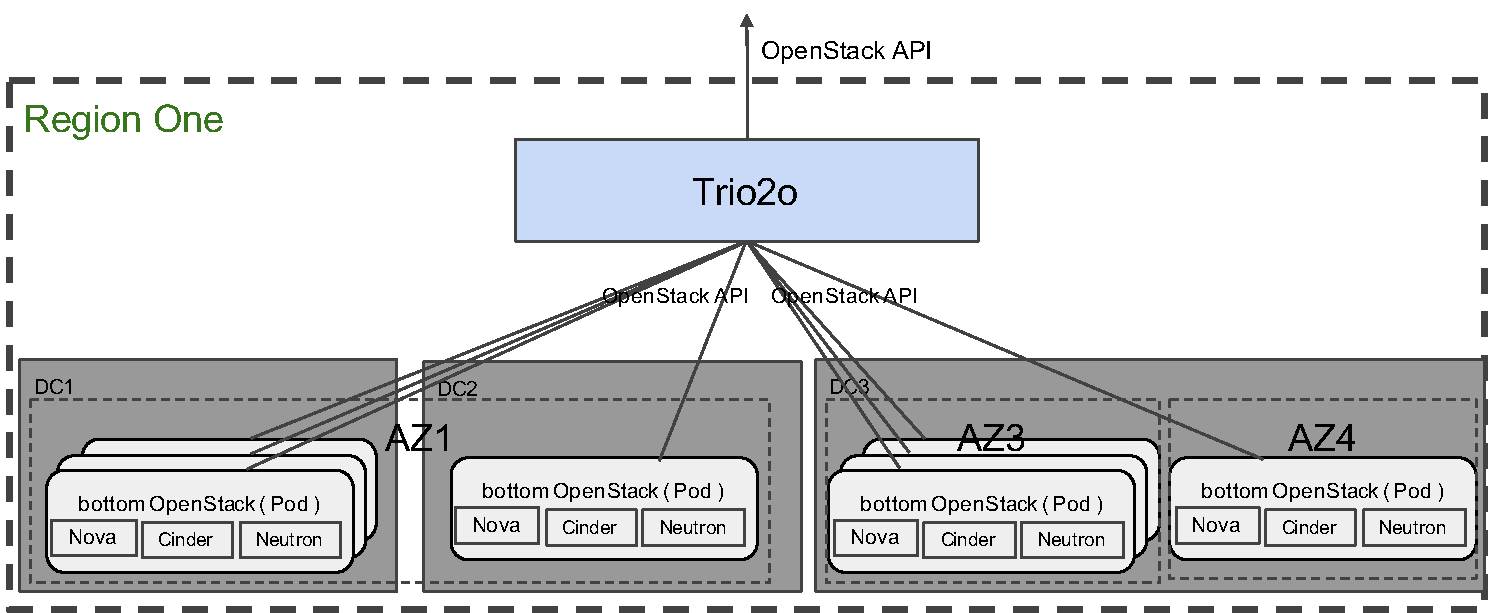
\includegraphics[width=0.5\textwidth]{trio2oarch}
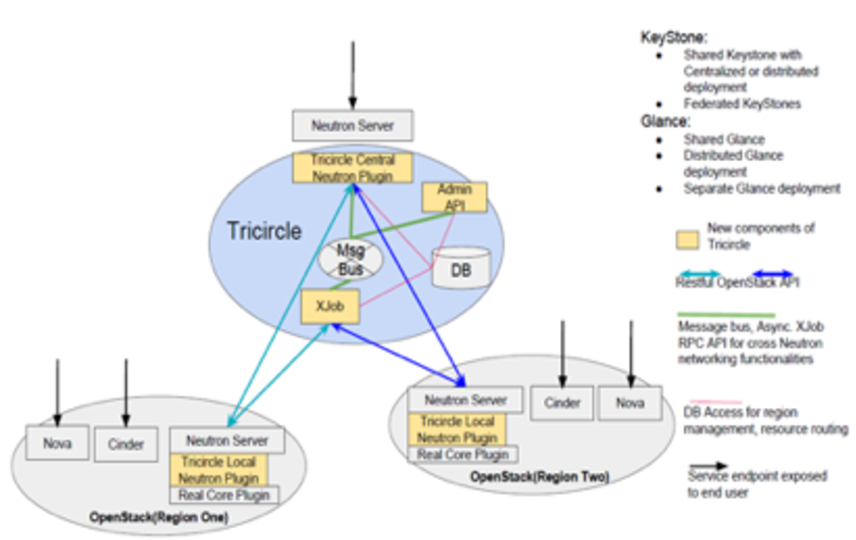
\includegraphics[width=0.5\textwidth]{tricirclearch}
\caption{High-level architecture of Trio2o \cite{Trio2oDesign} and TriCircle \cite{TriCircleDesign} }
\label{fig:Trio2oArch}
\end{center}
\end{figure}

Trio2o/Tricircle fulfills the requirements for Level 1 and 2. For level 3, a disconnected site will continue to run its workloads but it will not be possible to start new workloads on it until the disconnection is restored. All sites with connectivity with Trio2o/Tricircle will continue to operate normally. Level 4.1a is not an issue as the current implementation uses a shared glance across all sites. Trio2o leverages Tricircle for 4.1b and 4.1c while 4.1d is possible due to the global glance service. When it comes to 4.1e, it may be implemented as an Xjob job, provided that cross-region VM migration is supported natively by the bottom OpenStack instances (not currently supported). Level 4.1f may be supported provided that it is supported natively by the bottom OpenStack instances (not currently supported) while 4.1f is not supported. Levels 4.2  and 5 are mostly not yet supported in the current implementation, but there is nothing in the architecture that prevents this from it being realized. Level 6.a will not be an issue as long as the API version numbers are synchronized, but even with bottom sites having services with differing API versions, there is nothing in the design that prevents implementing such support. Level 6.b and 7 will be a challenge to implement due to the services that need to be shared across the several sites.  
\subsubsection{Kingbird}
\subsubsection{oaktree}



\subsection{Non-OpenStack approaches}
\label{subsec:non-os}




\subsection{Academic proposals}
\label{subsec:academic}





% 
\section{Discussions}
\label{sec:discussions}



\section{Related Work}
\AL{Should we have a related work Section}
\section{Conclusion}
\label{sec:conclusion}

The emergence of Network Function Virtualization (NFV) technologies as
well as Internet of Things (IoT) and Augmented/Virtual Reality (AR/VR)
applications herald a new era of Cloud Computing where infrastructures
need to leverage resources at the edge of the network in order to cope
with latency requirements.  Despite this growing need, there is no
cloud management system that is designed with such an infrastructure
in mind.

In this paper, we presented reflections to initiate discussions on this
hot topic. 
%[Dim] I'm not sure this sentence is correct:
We outlined a systematic grouping of the features that administrators/DevOps
expect and the requirements an edge infrastructure puts on a cloud management
system.
%e also identified existing efforts in this area and which may be used as a starting point to a full-blown solution.
We briefly studied the use of existing IaaS managers (\ie OpenStack)
to control an edge infrastructure highlighting the need for an
effective collaboration between the edge sites.  
We then discussed pros and cons of two possible strategies to follow when
designing a solution: (1) a \emph{top-down} approach which designs overlay
components that interact with underlying IaaS managers without modifying their
codebase; (2) a \emph{bottom-up} approach that extensively
improves existing software to fulfill the requirements. We concluded
that on the short-term, a \emph{top-down} approach is required to have
a timely working solution available. On a long-term, both approaches should be
considered simultaneously: \emph{bottom-up} to realize a native and efficient
system for the edge; \emph{top-down} to enable collaboration between different
cloud stacks (\eg OpenStack, Kubernetes).

Finally, it is noteworthy that our study lies on one kind of edge
infrastructure. Other variants can be envisioned where, for example,
hardware resources provided by third-party users can dynamically join
and leave the infrastructure. For such cases, this study needs to be
extended to integrate additional features not discussed in this paper.

%\AL{We should highlight that we conducted our study on one kind of  edge infrastructure. People start to envision more advanced scenarios where third party entities might provided hardware resources that can join the infrastructure. In such a case, our resource managmeent system will have to integrate additional features not discussed in the paper}



\bibliographystyle{acm}
{\footnotesize 
\bibliography{hotedge2018}}

\theendnotes

\end{document}







